% bare_jrnl_compsoc, texV1.4b, 2015/08/26, Michael Shell
\documentclass[10pt,journal,compsoc]{IEEEtran}

% *** MISC UTILITY PACKAGES ***

\newcommand{\note}[1]{\textcolor{magenta}{#1}} 
\usepackage[nocompress]{cite}
\usepackage[]{footmisc}
%\usepackage[notref, notcite]{showkeys}
\usepackage{hyperref} % autoref
% *** GRAPHICS RELATED PACKAGES ***
\ifCLASSINFOpdf
   \usepackage[pdftex]{graphicx}
  % declare the path(s) where your graphic files are
   \graphicspath{{./figures/}}
  % and their extensions so you won't have to specify these with
  % every instance of \includegraphics
  % \DeclareGraphicsExtensions{.pdf,.jpeg,.png}
\else
  % or other class option (dvipsone, dvipdf, if not using dvips). graphicx
  % will default to the driver specified in the system graphics.cfg if no
  % driver is specified.
   \usepackage[dvips]{graphicx}
  % declare the path(s) where your graphic files are
   \graphicspath{{./figures/}}
  % and their extensions so you won't have to specify these with
  % every instance of \includegraphics
   \DeclareGraphicsExtensions{.eps}
\fi

% latex, and pdflatex in dvi mode, support graphics in encapsulated
% postscript (.eps) format. pdflatex in pdf mode supports graphics
% in .pdf, .jpeg, .png and .mps (metapost) formats. Users should ensure
% that all non-photo figures use a vector format (.eps, .pdf, .mps) and
% not a bitmapped formats (.jpeg, .png). The IEEE frowns on bitmapped formats
% which can result in "jaggedy"/blurry rendering of lines and letters as
% well as large increases in file sizes.

% *** MATH PACKAGES ***
%% with other math-related packages, you may want to disable it.
\usepackage{amsmath, amsthm, amsfonts,amssymb,eulervm,xspace, mathtools}
\usepackage{stmaryrd}%mapsfrom 
\renewcommand{\restriction}{\mathord{\upharpoonright}} %restriction w/p space
\usepackage{mathrsfs} % math script fonts
\usepackage{relsize} %bigger
\usepackage{bm}
\theoremstyle{definition}
\newtheorem{definition}{Definition}[section]
\theoremstyle{remark}
\newtheorem{example}{Example}[section]
% *** SPECIALIZED LIST PACKAGES ***

\usepackage{xcolor}
\usepackage{algorithmic}
\usepackage[utf8]{inputenc}
\usepackage{subfig} %ieee does not like subfigure
\usepackage{multicol}
\usepackage{tikz}
\usetikzlibrary{cd} % commutative diagrams
\newtheorem{axiom}{Axiom}
\newtheorem{prop}{Proposition} %math?
\usepackage[switch]{lineno}
\renewcommand{\linenumberfont}{\normalfont\bfseries\small\color{lightgray}}
\usepackage{minted}
\setminted[python]{fontsize=\scriptsize, 
                   linenos,
                   numbersep=8pt,
                   autogobble, 
                   frame=lines,
                   framesep=3mm} 
% *** ALIGNMENT PACKAGES ***
\usepackage{array}
\usepackage{tabulary}
% IEEEtran contains the IEEEeqnarray family of commands

% *** SUBFIGURE PACKAGES ***
\ifCLASSOPTIONcompsoc
  \usepackage[caption=false,font=footnotesize,labelfont=sf,textfont=sf]{subfig}
\else
  \usepackage[caption=false,font=footnotesize]{subfig}
\fi

% *** FLOAT PACKAGES ***
\usepackage{dblfloatfix}

% *** PDF, URL AND HYPERLINK PACKAGES ***
\usepackage{url}

% *** Do not adjust lengths that control margins, column widths, etc. ***
% *** Do not use packages that alter fonts (such as pslatex).         ***
% There should be no need to do such things with IEEEtran.cls V1.6 and later.
% (Unless specifically asked to do so by the journal or conference you plan
% to submit to, of course. )

\usepackage[inline]{showlabels}

\usepackage{notation} %notation conventions
% correct bad hyphenation here
\hyphenation{}



\begin{document}
\linenumbers

\title{Topological Equivariant Artist Model for Visualization Library Architecture}
% author names and IEEE memberships
\author{Hannah~Aizenman, Thomas~Caswell, and~Michael~Grossberg,~\IEEEmembership{Member,~IEEE,}% <-this % stops a space
\IEEEcompsocitemizethanks{\IEEEcompsocthanksitem H. Aizenman and M. Grossberg are with the department of Computer Science, City College of New York. 
\protect\\
% note need leading \protect in front of \\ to get a newline within \thanks as
% \\ is fragile and will error, could use \hfil\break instead.
E-mail: haizenman@ccny.cuny.edu, mgrossberg@ccny.cuny.edu 
\IEEEcompsocthanksitem Thomas Caswell is with National Synchrotron Light Source II, Brookhaven National Lab 
\protect \\
E-mail: tcaswell@bnl.gov}% <-this % stops an unwanted space
\thanks{Manuscript received X XX, XXXX; revised X XX, XXXX.}
}


% for Computer Society papers, we must declare the abstract and index terms
% PRIOR to the title within the \IEEEtitleabstractindextext IEEEtran
% command as these need to go into the title area created by \maketitle.
% As a general rule, do not put math, special symbols or citations
% in the abstract or keywords.
\IEEEtitleabstractindextext{%
\begin{abstract}
The abstract goes here.
\end{abstract}

% Note that keywords are not normally used for peerreview papers.
\begin{IEEEkeywords}
%Computer Society, IEEE, IEEEtran, journal, \LaTeX, paper, template.
\end{IEEEkeywords}}


% make the title area
\maketitle


\IEEEpeerreviewmaketitle



\IEEEraisesectionheading{\section{Introduction}\label{sec:intro}}


\IEEEPARstart{T}

\section{Related Work}

\subsection{Topology}
The topological properties of visualization data are , as described by Wilkenson\cite{wilkinsonGrammarGraphics2005}. 

\begin{figure}[h!]
  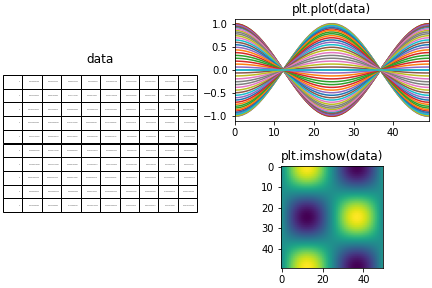
\includegraphics[width=1\columnwidth]{continuity.png}
\end{figure}
Visualization libraries designed around continuity,  
Visualization library algorithms assume 

\begin{figure}[h!]
  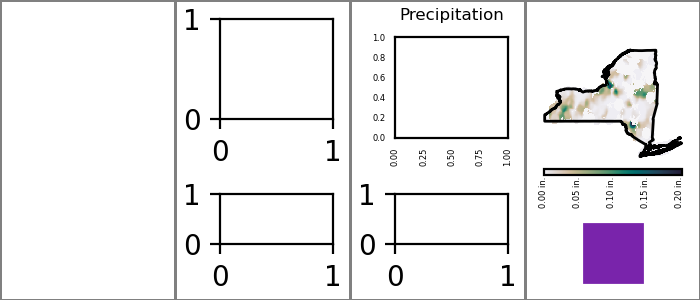
\includegraphics[width=1\columnwidth]{k_different_types.png}
\end{figure}
Fiber bundles are a mathematical structure that can be use to encode the topological properties of visualization data, as proposed by Butler\cite{butlerVectorBundleClassesForm1992,butlerVisualizationModelBased1989}. Broadly, fiber bundles

\subsection{Equivariance}


\section{Data And Visualizations}
\label{sec:atct}
\note{why why why?}
We use concepts from algberaic topolology and category theory to formally express the structure visualization components are expected to preserve.  Fiber bundles and sheaves, which come from algebraic topolology, provide a uniform generalizable way to describe data and visualizations. Category theory is a method to describe how objects are specified, constrained, and composed \cite{wielsManagementEvolvingSpecifications1998}\; therefore in this work we propose categorical constructions of visualization components as specifications for implementable components.

\subsection{Fiber Bundles}
\label{sec:atct:fiber-bundles}
Fiber bundles, are a "unified, dimension-independent framework", as described by Butler\cite{butlerVectorBundleClassesForm1992,butlerVisualizationModelBased1989}, that allow us to seperatly describe the topological properties and fields of a data source and also the mapping between topolology and data values. A fiber bundle $(\dtotalc, \dbasec, \pi, \dfiberc)$ is a structure with topological spaces $\dtotalc, \dfiberc, \dbasec$ and continuous surjective map $\pi: \dtotalc \rightarrow \dbasec$\cite{FiberBundle2020}. 

\begin{equation}[h]
  \label{eq:atct:fb:intro}
  \begin{tikzcd}[ampersand replacement=\&, row sep=huge]
   \dfiberc
    \arrow[r, hook, color=total] \& 
    \dtotalc
    \arrow[d, "\pi"',color=total] \\
     \& 
  \dbasec
     \arrow[u, "\dsectionc"', bend right, pos=.5, color=section]
  \end{tikzcd}
\end{equation} 

The \textcolor{base}{base space} is a topological space \dbasec\ with points $\dbasepointc \in \dbasec$ and topology $\mathcal{T}_{\dbasec}$; $\mathcal{T}_k$ is a set of opensets $ \dbasepointc \in \opensetc \subseteqq \dbasec$ \cite{munkresElementsAlgebraicTopology1984} that cover the base space \dbasec.  The \textcolor{fiber}{fiber space} is a topological space \dfiberc\ that is the preimage of the projection function $\pi$ at a point in the base space $\dfiber_{\dbasepointc} = \pi^{-1}(\dbasepointc)$ and fibers of a bundle are isomorphic $\dfiberc \simeq \dfiberc_{\dbasepointc}\;\forall \dbasepointc \in \dbase$. The \textcolor{section}{sections} of a bundle $\dsection$ are maps from the base space to points in the bundles over that base space $\textcolor{set}{\Gamma}$ denotes the set of all sections in a bundle over an openset. 
\begin{equation}
  \label{eq:atct:fb:sections}
  \cgamma{\opensetc}{\dtotalc\restriction_{\opensetc}} \coloneqq \big\{\dsectionc: \opensetc\rightarrow \dtotalc\restriction_{\opensetc} \; \bigm{\vert} \pi(\dsectionc(\dbasepointc)) = \dbasepointc\;for\, all\; \dbasepointc \in \opensetc \big\} 
\end{equation}
 
A fiber bundle is locally trivial, which means that for every point \dbasepointc\ there exists an open neighborhood $\dbasepointc \in \opensetc \subseteq \dbasec$ such that there is a homeomorphism $\pi^{-1}(\opensetc)\xrightarrow{\equivc} \opensetc \times \dfiberc$. A bundle may be globally trivial, meaning that $\dtotalc = \dbasec \times \dfiberc$, and generally can be thought of as a twisted product of total and base spaces \cite{munkresElementsAlgebraicTopology1984}. Throughout this work we will assume that fiber bundles are trivial because that allows us to model the section functions as from $\texttt{base} \rightarrow \texttt{fiber}$ since the fiber is the same at all points in the base space. 

Fiber bundles can be used to model data for visualization, as proposed by Butler\cite{butlerVectorBundleClassesForm1992, butlerVisualizationModelBased1989}. We describe the topological properties of the data \cite{wilkinsonGrammarGraphics2005} as the base space \dbasec. The topological properties, as described by Wilkenson, are how the data is organized - for example \dbase\ could be discrete points, a line, a 2D surface, a 3D volume, or a graph. The names and data types of the data fields can be expressed as the fiber space \dfiberc, as described by Spivak \cite{spivakDatabasesAreCategories2010,spivakSIMPLICIALDATABASES}. Extending Spivak's fiber bundle description of a table, we define the values returned by a section as named and typed records of the dataset. 

\begin{figure}[h!]
  \label{fig:atct:fb}
  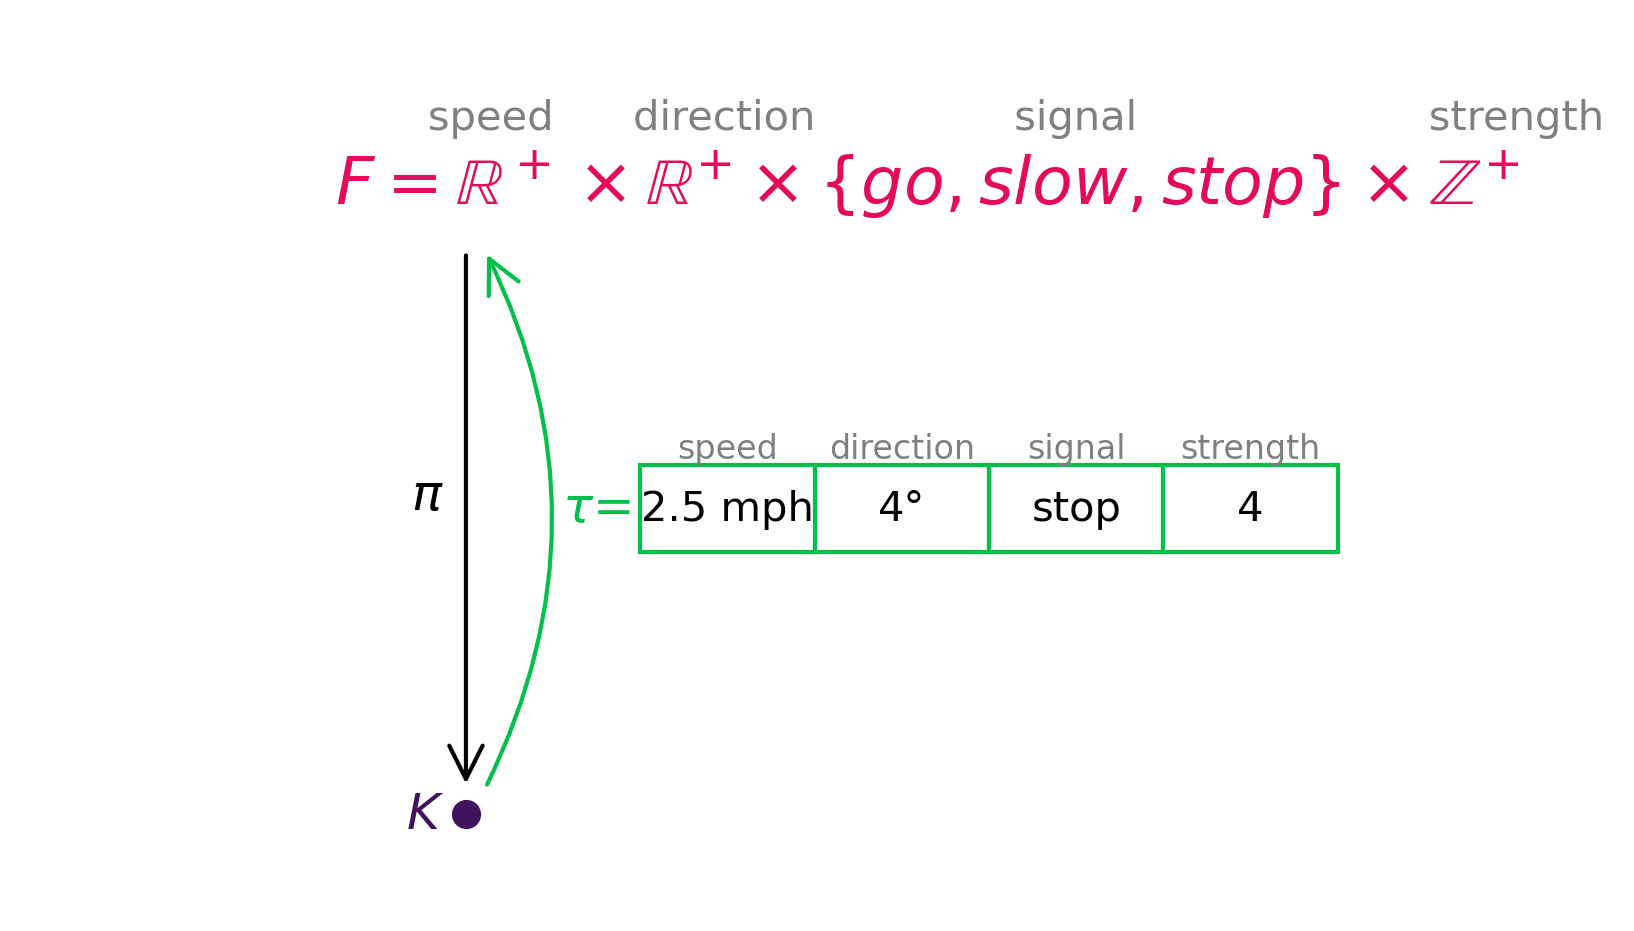
\includegraphics[width=\columnwidth]{fb_tau.png}
  \caption{This trivial dataset consists of a single point $\dbasec$ and the fields \texttt{speed, direction, signal, and strength}. Each of these fields has an associated datatype, which is the set of possible valid values for that field. The fiber space is the cartesian product of these sets $\dfiberc$. Each section $\dsectionc$ function returns a single record in the fiber, here the data record outlined in green.  
  \note{maybe change to temperature}}
\end{figure} 
A fiber bundle is a mathematical structure for encoding continuity, type, and datasets with that continuity and type. In \autoref{fig:atct:fb}, the continuity is a discrete point \dbase. The fiber space that encodes the types is the cartesian product of the field types, and the section returns a single record with values of each field type. While this is a very trivial example, a fiber bundle base space can have almost any topology. The fiber space also does not really have restrictions on which types it can encode or the structure of those types - for example, \texttt{speed} and \texttt{direction} are separate fibers in \autoref{fig:atct:fb} but can be combined into a single two dimensional fiber $\dfiber_{speed, direction} = {\mathbb{R}^{+}}^{s}$ The generality in base space and fiber space makes fiber bundles a unified dimension and type independent data abstraction that can encode most of the common visualization data set structures, such as continuous functions, tables, data cubes, images and networks. 

We also use fiber bundles to represent the output of a visualization algorithm, which we term the graphic but generalizes to output on any display space, such as a screen or 3D print. 
\begin{equation}
  \label{eq:atct:fb:graphic}
  \gfiberc \hookrightarrow \gtotalc \xrightarrow{\pi} \gbasec
\end{equation}
The base space \gbasec\ is a parameterization of the display area, for example the inked bounding box in cairo \cite{CairographicsOrg}. The fiber space \gfiberc\ is an abstraction of the renderer fields, for example $\{x,\,y,\,r,\,g,\,b,\,a\}$. The sections of the graphic 
\begin{equation}
  \label{eq:atct:fb_graphic_section}
  \cgamma{\opensetgc}{\gtotalc\restriction_{\opensetgc}} \coloneqq \big\{\gsectionc: \opensetgc\rightarrow \gtotalc\restriction_{\opensetgc} \; \bigm{\vert} \pi(\gsectionc(\gbasepointc)) = \gbasepointc\;for\, all\; \gbasepointc \in \opensetgc \big\}
\end{equation}
are functions that generate different graphics, for example markers for a scatter plot, bars for a bar chart, cells of a heatmap, or pixels of an image.


\begin{figure}[h!]
  \label{fig:atct:fb:graphic}
  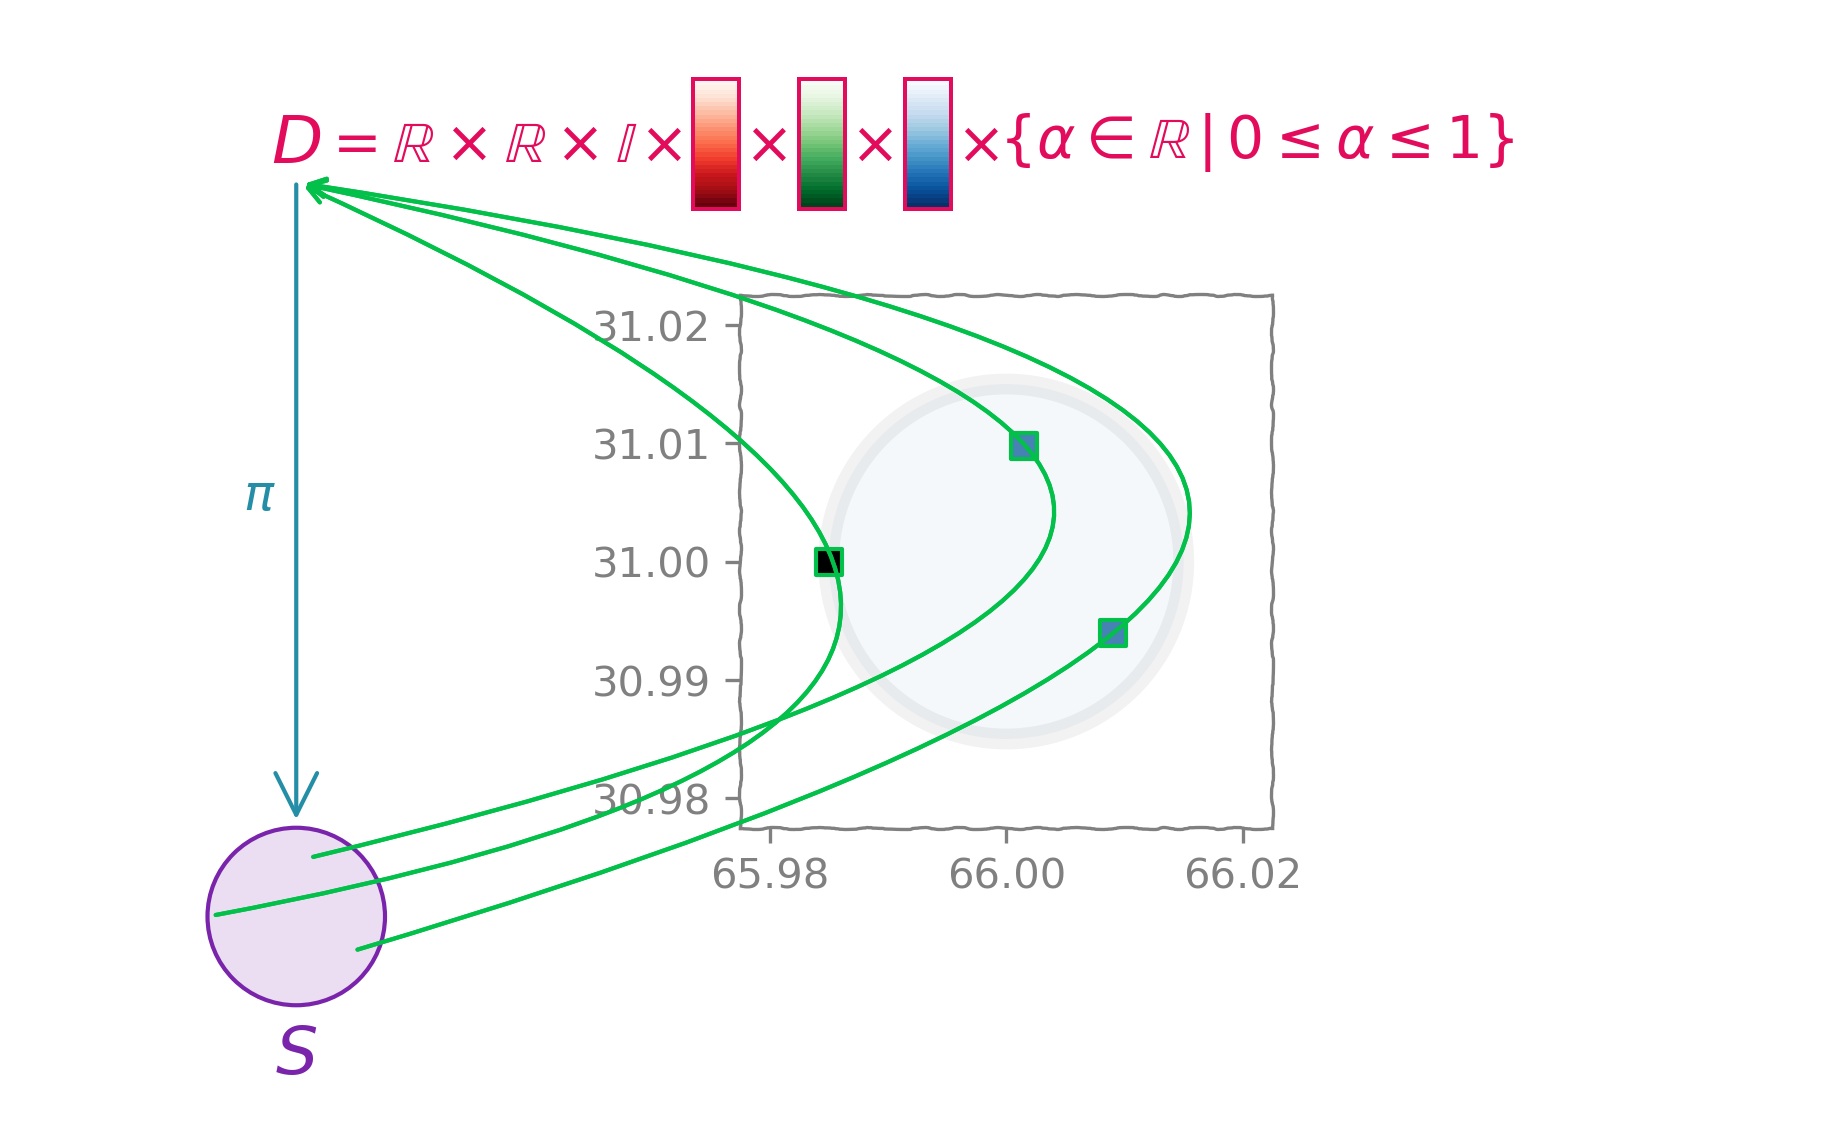
\includegraphics[width=1\columnwidth]{fb_rho.png}
  \caption{A bundle representation of a section that generates a scatter marker on a 2D screen. The fiber space encodes the potential color and position of each pixel in a prerender space. The marker is a 2d graphic; therefore the base space that parameterizes the graphic area \dbasec\ is a 2d disc. This section \gsection\ describes how to build a square red marker; a section evaluated on a single point $\gbasepoint \in \gbase$ is an infinitesimally small piece of the square, here illustrated as the small piece of the square outlined in green.  }
\end{figure}

In \autoref{fig:atct:fb:graphic}, the section function $\gsection$ encodes the drawing of a red square marker. The renderer subsamples the position fibers  \textit{x} and \textit{y} of the graphic fiber space \gfiber. The preimage of the section at these coordinates returns a set of coordinates ${\gsection^{-1}_{x,y}} = \{\gbasepoint | \gsection(\gbasepoint)\restriction_{x,y} = \(x,y\)\}$ at the points $\gbasepoint \in \gbase$ in the graphic base topological space. The section is then evaluated at these points $\gsection\restriction_{\gsection^{-1}_{x,y}}$ to return a set of points in the fiber. One of these points, enlarged for visibility, is illustrated as the small square swatch inside the larger marker in \autoref{fig:atct:fb}. The renderer is handed some version of $\gsection$ to produce the final graphic. 

\subsection{Input and Output Types}
\label{sec:atct:io}
As described in \autoref{sec:atct:fiber-bundles}, we model data as a map from base space to fiber space.To encapsulate the structure carried in these maps, and provide a way to define these maps in reusable and composable manner, we define categories of base and fiber spaces. 

\begin{definition}
  \label{sec:atct:io:base}
  The base space category $\mathcal{\opensetc}$ has open set objects $\opensetc$ and inclusion morphisms $\iota: \opensetc_1 \rightarrow \opensetc_2$ such that $\opensetc_1 \subseteq \opensetc_2$. 
\end{definition}

By definition, each object in a category has an identity morphism and morphisms are associative and commutative \cite{barrCategoryTheoryComputing}. 

\begin{definition}
  \label{def:atct:io:fiber}
  The fiber category $\mathcal{\dfiberc}$ is a monoidal category, meaning the category has a single object $\dfiberc$ of an arbitrary type. The morphisms on the fiber object are $\dfunctc \in Hom(\dfiberc, \dfiberc)$. 
\end{definition}

The fiber category is equipped with a bifunctor $\otimes: \mathcal{\dfiber} \times {\dfiber}$. The bifunctor provides a method for combining fibers, thereby allowing for fields that contain multityped values. For example, RGB color can either be represented as three fiber fields $\dfiber_{red}, \dfiber_{green}, \dfiber_{blue}$ or a composite fiber field $\dfiber_{red} \otimes \dfiber_{green} \otimes \dfiber_{blue} = \dfiber_{RGB}$.

\subsection{Sheaves}
\label{sec:atct:sheaves}
Sheaves on bundles are an "algebraic data structure", as described by Ghrist \cite{ghristElementaryAppliedTopology2014}, for expressing the bookkeeping involved in keeping track of sections of data over opensets. Sheaves are a way of expressing that subsets, distributed data, and streaming data are local sections that can be glued together. Formally, pre-sheaves are functors, meaning they are functions from objects of one category to objects of another category \cite{WhatFunctorDefinitions}. Here the sheaf 
\begin{equation}
  \sheafc_{\dbasec, \dtotalc}: \opensetc \rightarrow \cgamma{\opensetc}{\dtotalc\restriction_{\opensetc}}
\end{equation}
denotes a sheaf from opensets on the base space $\dbase$ to sets of sections on the bundle $\dtotal$. As a contravariant functor it preserves morphism s

\begin{equation}
  \label{eq:atct:presheaf}
  \begin{tikzcd}
    \cgamma{\opensetc_1}{\dtotalc\restriction_{\opensetc_1}}  &  & \cgamma{\opensetc_2}{\dtotalc\restriction_{\opensetc_2}} 
    \arrow[ll, "\iota^*"', maps to, color=set] \\
    & & \\
    \opensetc_1 
    \arrow[rr, "\iota", maps to, color=base] 
    \arrow[uu, "{\sheafc_{\dbasec, \dtotalc}}", maps to, color=sheaf] &  & \opensetc_2 
    \arrow[uu, "{\sheafc_{\dbasec, \dtotalc}}"', maps to, color=sheaf]              
    \end{tikzcd}
\end{equation}

which associates a set of sections $\cgamma{\openset}{\dtotal\restriction_{\openset}}$ with an openset \openset. The sets of sections are objects of the category \setc\ and the morphisms of the category are restrictions\footnote{restriction functions } $\iota^*$. The sheaf over a an open set $\openset$ surrounding a point $\dbasepoint$ is called a stalk\cite{StalkSheaf2019}
\begin{equation}
  \label{eq:atct:sheaf:stalk}
    \sheaf_{\dbase, \dtotalc}\restriction_{\dbasepoint}\coloneqq \lim\limits_{\openset\ni \dbasepoint} \Gamma(\openset, \dtotal\restriction_{\openset}) 
\end{equation}
where the fiber is contained inside the stalk  $\dfiber_{\dbasepoint} \subset  \sheaf_{\dbase, \dtotal}\restriction_{\dbasepoint}$. The germ is the section evaluated at a point in the stalk  $\dsection(\dbasepoint) \in \sheaf_{\dbase, \dtotal}\restriction_{\dbasepoint}$ and is the data. \note{I never use stalk and germ terminology at any point in this paper}
 
A sheaf is a presheaf that satisfies the locality and gluing axioms \cite{bakerMathsSheaf}. 
\begin{definition}
\label{def:atct:sheaf:locality}
The locality axiom is that given a union of opensets $\mathscr{\opensetc} = \bigcup\limits_{i\in I} \opensetc_i$ and $\dsectionc^{a}, \dsectionc^{b} \in \sheafc(\mathscr{\opensetc})$,  if $\dsectionc^{a}\restriction_{\opensetc_i} = \dsectionc^{b}\restriction_{\opensetc_i}$ for each $\opensetc_i \in \opensetc$ then $\dsectionc^{a} = \dsectionc^{b}$
\end{definition}
This means that two sections in a sheaf are equal when they evaluate to the same values over all open sets in a collection. 
\begin{definition}
\label{def:atct:sheaf:gluing}
The gluing axiom is that given $\dsectionc^{i} \in \sheafc(\opensetc_i)$ such that ${\dsectionc^{i}}\restriction_{\opensetc_i\cap \opensetc_j} = {\dsectionc^{j}}\restriction_{\opensetc_i \cap \opensetc_j}$ for $\opensetc_i, \opensetc_j \in \mathscr{\opensetc}$, there exists $\dsectionc \in \sheafc(\mathscr{\opensetc})$ such that $\dsectionc\restriction_{\opensetc_i} = {\dsectionc^{i}}$. 
\end{definition}
This means we can construct a section $\dsection$ on the collection of open sets that is the union of sections defined on specific open sets. This expresses an equivalency between a concatenated representation of data and the distributed representation of the same data. In this model, we represent data and graphics as a sheaf; doing so allows us to express that data sources are expected to have the bookkeeping that a sheaf requires, meaning inclusions, restrictions, locality, and gluing must be preserved. 

\subsubsection{Structure on Data}
\label{sec:atct:sheaves:measurments}
We define structure on data as the allowable \textcolor{action}{transformations on the bundle}, which we formalize as actions $\dfuncc$ on sections of that sheaf. Our construction of $\dfunc$ is a generalization of the classification of measurement scales by their mathematical structure \cite{stevensTheoryScalesMeasurement1946,leaFormalizationMeasurementScale, thomasMathematizationNotMeasurement2014}, which often serves as the basis of the equivariance described in \autoref{sec:related-work:equivariance}.

We separate data transformations into two types, transformations on the base space $(\dfunchc, \dfuncpullc)$ and transformations on the fiber space $\dfunctc$. 
\begin{equation}
  \label{eq:atct:sheaves:monoid_morphism}
  \begin{tikzcd}
    \cgamma{\opensetc}{\dtotalc\restriction_{\opensetc}} 
    \arrow[rr, "\dfuncpullc", color=action, maps to] &  & 
    \cgamma{\opensetc^{\prime}}{\dfuncpullc\dtotalc\restriction_{\opensetc^{\prime}}} & 
    \cgamma{\opensetc^{\prime}}{\dfuncpullc\dtotalc\restriction_{\opensetc^{\prime}}} 
    \arrow[dd, "\dfunctc", color=action] \\
     &  & &       \\
    \opensetc 
    \arrow[uu, maps to,color=sheaf]  &  & \opensetc^{\prime} 
    \arrow[ll, "\dfunchc"', color=action, maps to] 
    \arrow[uu, maps to, color=sheaf] & \cgamma{\opensetc^{\prime}}{\dfuncpullc\dtotalc\restriction_{\opensetc^{\prime}}}                       
    \end{tikzcd}
\end{equation}
As shown in \autoref{eq:atct:sheaves:monoid_morphism}, the base space transform 
\begin{equation}
 \label{eq:atct:morphism:base}
\dfunch: \openset^{\prime}\rightarrow \openset
\end{equation}
is from one open set to another open set in the same base space $\openset, \openset^{\prime} \subseteq \dbase$. For example a remapping of an underlying indexing, such as a sorting of primary keys for a database of discrete values. This base space transformation induces a pullback section 
\begin{equation}
  \label{eq:atct:morphism:basepull}
  \dfuncpull \dsection \restriction_{\openset^{\prime}}: \dsection\restriction_{\openset^{\prime}} \mapsto \dsection \restriction_{\openset^{\prime} \circ \dfunch} 
\end{equation}
such that $\dsection|_{\openset} = \dfuncpull\dsection|_{\opensetc^{\prime}}$ because $\dsection|_{\openset} = \dsection|_{\dfunch(\opensetc^{\prime})}$. This means that the base space transformation \dfunch\ does not change the data values at a given point
\begin{equation}
  \label{eq:atct:morphism:verify_base}
  \dsection(\dbase) = \dfuncpull\dsectionc(\dbasepoint^{\prime}) = \dsection(\dfunch(\dbase^{prime}))
\end{equation} 
where $\dfunch(\dbasepoint^{\prime}) = \dfunch(\dbasepoint)$. As introduced in \autoref{def:atct:io:fiber}, the fiber transformation $\dfunct: \dfuncpull \dtotal_{\dbasepoint^{\prime}} \rightarrow \dfuncpull \dtotal_{\dbasepoint^{\prime}}$ is a morphism on the fiber $\dfunct \in Hom(\dfuncpull\dfiber\restriction_{\dbasepoint^{\prime}},\dfuncpull\dfiber\restriction_{\dbasepoint^{\prime}})$ restricted to a point $\dbasepoint^{\prime} \in \openset^{\prime}$. The fiber transformation is a change in section 
\begin{equation}
  \label{eq:atct:morphism:fiber}
  \dfunct: \dfuncpull \dsection \restriction_{\openset^{\prime}} \mapsto \dfuncpull \dsection^{\prime} \restriction_{\openset}
\end{equation}
where $\dsection, \dsection^{\prime} \in \Gamma(\openset^{\prime}, \dfuncpull\dtotal\restriction_{\openset^{\prime}})$. Examples of a fiber transformation are actions such as partial ordering for ranking purpose \cite{bruggemannRankingPrioritizationMultiindicator2011} and the permutation, ordering, translation, and scaling codified as Steven's measurement scales \cite{stevensTheoryScalesMeasurement1946}. 

We define a full data transformation as one that induces both a remapping of the index space and a change in the data values
\begin{equation}
  \label{eq:atct:morphism:all}
  \dfuncc: \dsectionc\restriction_{\opensetc} \mapsto \dsectionc^{\prime}\restriction_{\opensetc} \circ \dfunchc
\end{equation}
which gives us an equation that can express complex transformations. For example, wind vectors on a sphere are a non-trivial bundle, meaning their fibers aren't identical at every point in the base space; therefore a rotation (change of base space) of the sphere must include an adjustment to the values that have moved closer to the pole (a change in fiber).  
The data transform \dfunc\ is composable 
\begin{equation}
  \dfuncc = (\dfunchc, \prod\limits_{i=0}^{n}\dfunctc_i)
\end{equation}
if each (identical) component base space is transformed in the same way $\dfunch$ and there exists functions $\dfunc_{a,b}: \dtotal_a \times \dtotal_b \rightarrow \dtotal_a \times \dtotal_b$, $\dfunc_{a}: \dtotal_a \rightarrow \dtotal_a$ and $\dfunc_{b}: \dtotal_b \rightarrow \dtotal_b$ such that $\pi_a \circ \dfunc_a = \dfunc_{a,b} \circ \pi_a$ and $\pi_b \circ \dfunc_b = \dfunc_{a,b} \circ \pi_b$ then $\dfunc_{a,b} = (\dfunc_a, \dfunc_b)$. This allows us to define a data transform where each fiber transform $\dfunct_{i}$ can be applied to a different fiber field $\dfiber_i$. 

\begin{figure}[h!]
  \label{fig:atct:phi}
  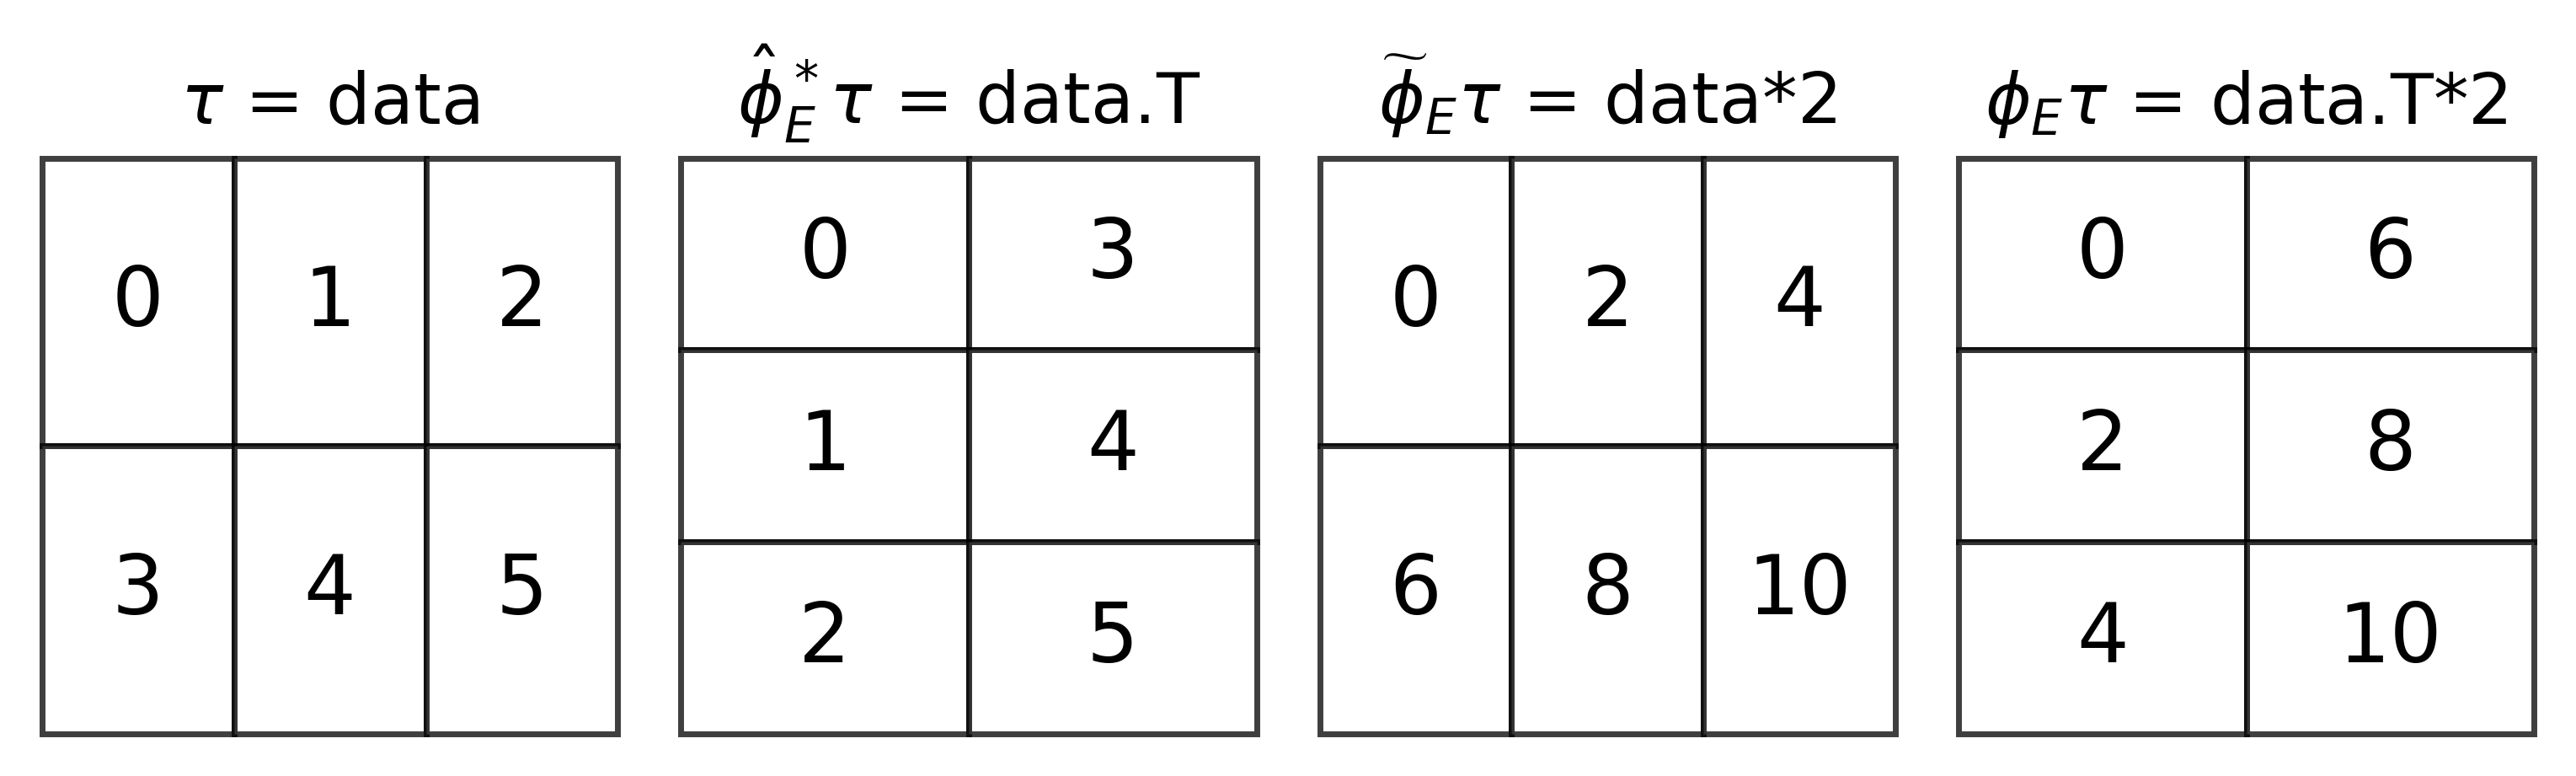
\includegraphics[width=\columnwidth]{phi.png}
  \caption{Values in a data set can be transformed in three ways: $\dfunch$-values can change position, .e.g transposed;  $\dfunct$-values can change, e.g. doubled; $\dfunc$ - values can change position and value}
\end{figure}
\autoref{fig:atct:phi} provides an example of a base space change \dfunch, a fiber space change \dfunct, and a composition of the two \dfunc\ applied to each data point $x_{\dbasepoint} \in \texttt{data}$. As defined in \autoref{eq:atct:morphism:verify_base}, 
since transposition is a $(\dfunch, \dfuncpull)$, every data value $x_{\dbasepoint}$ must be equal to the value at the corresponding location in the transposed matrix $x_{\dbasepoint} = x_{\dbasepoint^{\prime}}, \dfunch(\dbasepoint^{\prime}) = \dbasepoint$ for all $x_{\dbasepoint^{\prime}} \in texttt{data.T}$ . In \autoref{fig:atct:phi}, this is demonstrated in the columns becoming rows such that there are no new values and each value retains the same neighboring values. As defined in \autoref{eq:atct:morphism:fiber} scaling is a transform $\dfunct$ that changes the value of each point but not its location. In \autoref{fig:atct:phi}, this means that $x_{\dbasepoint^{\prime}}= 2*x_{\dbasepoint}, \dbasepoint = \dbasepoint_{\prime}$ for all indices in \textt{data}, \textt{data.T}. As defined in \autoref{eq:atct:morphism:all} and illustrated in \autoref{fig:atct:phi}, these transformations can combine to yield a matrix that is both transposed and scaled such that $x_{\dbasepoint^{\prime}} = 2*x_{\dbasepoint}$ for all  
$\dfunch(\dbasepoint^{\prime}) = \dbasepoint$

\subsection{Maps Between Spaces}
The data sections defined in \autoref{eq:atct:fb} are sections of sheaves, introduced in \autoref{sec:atct:sheaves}, over open sets $\openset \subseteq \dbase$ in a base space \dbase\ that encodes the topology of the data topology. The graphic sections, defined in \autoref{eq:atct:fb_graphic_section}, are sections of sheaves over open sets $\opensetg \subseteq \gbase$ in a base space \gbase\ that encodes the topology of the graphic. We propose that there exists a continuous \textcolor{functor}{map between topological spaces} \vindexc 
\begin{equation}
  \label{eq:atct:xi}
  \vindexc: \opensetgc \rightarrow \opensetc 
\end{equation}
such that every $\opensetg \subseteq \gbase$ must map to a corresponding set $\openset \subset \dbase$. 

Given the map between spaces \vindex\, a property of sheaves is that there exist image functors\cite{ImageFunctorsSheaves2021} functors \vindexpull\ and \vindexpush. The \textcolor{functor}{pullback functor} $\vindexpullc$ sends sheaves over $\dbase$ to $\gbase$ and the \textcolor{functor}{pushforward functor} $\vindexpushc$  sends sheaves over $\gbase$ to $\dbase$
\begin{equation}
  \label{eq:atct:morphisms:xi}
\begin{tikzcd}[row sep=huge]
  \cgamma{\opensetc}{\dtotalc\restriction_{\opensetc}} 
  \arrow[rr, "\vindexpullc", maps to, color=functor] &  & 
  \cgamma{\opensetgc}{\vindexpullc\dtotalc\restriction_{\opensetgc}}  \\
  \opensetc 
  \arrow[d, "{\vindexpushc\sheafc_{\gbasec,  \gtotalc}}", dashed, maps to, color=sheaf] 
  \arrow[u, "{\sheafc_{\dbasec, \dtotalc}}"', maps to, color=sheaf] &  & 
  \opensetgc 
  \arrow[d, "{\sheafc_{\gbasec, \gtotalc}}", maps to, color=sheaf] 
  \arrow[u, "{\vindexpullc\sheafc_{\dbasec, \dtotalc}}"', dashed, maps to, color=sheaf] 
  \arrow[ll, "\vindexc"', maps to, color=functor] \\
  \cgamma{\opensetc}{\vindexpushc\gtotalc\restriction_{\opensetc}} &  & 
  \cgamma{\opensetgc}{\gtotalc\restriction_{\opensetgc}} 
  \arrow[ll, "\vindexpushc"', maps to, color=functor]                                                         
  \end{tikzcd}
\end{equation}
such that there is an association between graphic sections \gsection\ that take as input \gbasepoint\ and data sections that take input \dbasepointc\ when $\vindex(\gbasepoint) = \dbasepoint$. 

The pull back $\vindexpullc$ transports sheaves of sections on $\openset \subseteq \dbase$ over $\opensetg \subseteq \gbase$
\begin{equation}
  \vindexpullc\dsectionc: \opensetgc \rightarrow \vindexpullc \dtotalc\restriction_{\opensetgc} \in \cgamma{\opensetgc}{\vindexpullc\dtotalc\restriction_{\opensetgc}} 
\end{equation}
such that there is a way to then look up what data values correspond with a graphic index
\begin{equation}
  \vindexpullc\dsectionc(\gbasepointc) = \dsectionc(\vindex(\gbasepointc)) = \dsectionc(\dbasepointc)
\end{equation}

 The pushforward $\vindexpushc$ transports sheaves of sections on $\opensetgc$ over $\openset$
 \begin{equation}  
  \vindexpushc\gsectionc: \opensetc \rightarrow \vindexpushc \gtotalc\restriction_{\opensetc} \in \cgamma{\opensetc}{\vindexpushc\gtotalc\restriction_{\opensetc}} 
\end{equation}
such that it provides a way to look up which graphic  corresponds with a data index
\begin{equation}
  \vindexpushc\gsectionc(\dbasepointc) = \gsectionc\restriction_{\vindexprec(\dbasepointc)} = \gsectionc(\gbasepointc)\;\forall \gbasepointc\in \vindexprec(\dbasepointc)
\end{equation}

Therefore, the continuous map $\vindex$ and transport functors $\vindexpull, \vindexpush$ allow us to express the correspondence between graphic section and data section. 

\begin{figure}[h!]
  \label{fig:atct:morphisms:sheaf}
  \includegraphics*[width=1\columnwidth]{xi_scatter.png}
  \caption{The base space functor $\vindexc$ is the mapping from each disc $\gbasec_i$ to it's corresponding point $\dbasepointc_i$. Over each point is a data record $\dsectionc$. The pullback function $\vindexpullc$ copies these records over $\gbase$ so that each piece of each marker knows the data associated with it. Each graphic disc has a corresponding graphic function $\gsectionc$. The pushforward function $\vindexpushc$ converts $\gsectionc$ into the visual parameters associated with each data point $\dbasepoint$.}
\end{figure}

Functors between sheaves are a way of expressing the bookkeeping involved in keeping track of which graphic section corresponds to which data section. This allows us to construct graphic specifications for each data index $\vindexpush\gsection$ and retrieve the data $\vindexpull\dsection$ for any graphic section generating any piece of a graphic. In \autoref{fig:atct:morphisms:sheaf}, the graphic specifications are the set of visual parameters associated with each point $\dbasepoint_i$. Each of these parameters describes the corresponding graphic $\gsectionc|_{\gbase_i}$ generated by evaluating the graphic section on the graphic base space associated with that data point $\vindexpre^{\dbasepoint_i} = \gbase_i$. The pullback functor $\vindexpull$ copies each data section at each point $\dsectionc(\dbasepointc_i)$ over the corresponding disk; in \autoref{fig:atct:morphisms:sheaf} this means that every pixel in a given marker, for example the yellow triangle, maps back into a single data record. Visualization specification languages such as vega \cite{heerDeclarative2010} and svg \cite{quintScalable2003} assume that there is a graphic  specification for every point. Interactive tooltips assume that there is a map between the graphics rendered on screen and the data such that a glyph maps back to a record. The functors $(\vindex, \vindexpush, \vindexpull)$ codify the expectation of these mappings between data and graphic space. 

We propose that visualization libraries implement morphisms from a data sheaf $\sheafc_{\dtotal, \dbase}$ to a graphic sheaf $\sheafc_{\gtotal, \gbase}$ 
\begin{equation}
  \label{eq:atct:sheaves:homset}
  \begin{tikzcd}
    \cgamma{\opensetc}{\dtotalc\restriction_{\opensetc}} 
    \arrow[dd, "\textcolor{set}{Hom}_{\sheafc_{\dbasec}}"', color=homset] 
    \arrow[rrdd, "\textcolor{set}{Hom}_{\sheafc_{\dbasec},\sheafc_{\gbasec}}", color=homset] 
    \arrow[rr, "\vindexpullc", color=functor] &  &
    \cgamma{\opensetgc}{\vindexpullc\dtotalc\restriction_{\opensetgc}} 
    \arrow[dd, "\textcolor{set}{Hom}_{\sheafc_{\gbasec}}", color=homset] \\
     & & \\
    \cgamma{\opensetc}{\vindexpushc\gtotalc\restriction_{\opensetc}} &  & 
    \cgamma{\opensetgc}{\gtotalc\restriction_{\opensetgc}} 
    \arrow[ll, "\vindexpushc"', color=functor]                  
    \end{tikzcd}
\end{equation}
and the hom set is the set of all morphisms from one sheaf to the other. The functors $\vindexpullc, \vindexpushc$ are adjoint, meaning that there is a functorial isomorphism \cite{harder2008lectures} such that 
\begin{equation}
  \label{eq:atct:sheaves:homset:functors}
\begin{split}
  & \textcolor{set}{Hom}_{\sheafc_{\gbasec}}(\vindexpullc\sheafc_{\dtotalc, \dbasec},\sheafc_{\gtotalc,\gbasec})\\
  \simeq & \textcolor{set}{Hom}_{\sheafc_{\dbasec}}(\sheafc_{\dtotalc, \dbasec},\vindexpushc\sheafc_{\gtotalc,\gbasec}) \\
  \simeq & \textcolor{set}{Hom}_{\sheafc_{\dbasec},\sheafc_{\gbasec}}(\sheafc_{\dtotalc, \dbasec},\sheafc_{\gtotalc,\gbasec}) \\
\end{split} 
\end{equation}
which means that the diagram of sheaf morphisms \autoref{eq:atct:sheaves:homset} is commutative; therefore the functors $\vindexpullc$ and $\vindexpushc$ can be used to adapt morphisms written over one space to another space. 
This provides us flexibility over which space to construct data to graphic transforms. For example, specifications such as svg\cite{quintScalable2003} and Vega\cite{satyanarayanDeclarativeInteractionDesign2014}, typically define their transformations in data space and return specifications for the render to evaluate. An artist may also want to specify the transformations in a proxy of graphic space, for example for operations like dynamic resampling \note{citation:root maybe}. 


\section{Artist: Data to Graphic}
\label{sec:artist}
In this work we propose that visualization libraries are implementing a subset of the functions in the hom sets in \autoref{eq:atct:sheaves:homset} and we call these subset of functions the artist:
\begin{align}
  \label{eq:artist:hom_transport}
  \vartistc:& \cgamma{\opensetc}{\dtotalc\restriction_{\opensetc}}\textcolor{artist}{\rightarrow} \cgamma{\opensetgc}{\gtotalc\restriction_{\opensetgc}} \in \textcolor{set}{Hom}_{\sheafc_{\dbase}, \sheafc_{\gbase}}\\
  \vartistc^{\dbasec}:&\cgamma{\opensetc}{\dtotalc\restriction_{\opensetc}}  \textcolor{artist}{\rightarrow} \cgamma{\opensetc}{\vindexpushc\gtotalc\restriction_{\opensetc}} \in \textcolor{set}{Hom}{\sheafc_{\dbase}}\\
  \vartistc^{\gbasec}:& \cgamma{\opensetgc}{\vindexpullc\dtotalc\restriction_{\opensetgc}} \textcolor{artist}{\rightarrow} \cgamma{\opensetgc}{\gtotalc\restriction_{\opensetgc}} \in \textcolor{set}{Hom}_{\sheafc_{\gbase}}
\end{align}
 Because the artists can be constructed as morphisms of sheave over the same base spaces, as listed in \autoref{eq:atct:sheaves:homset:functors}, they are natural transformations
\begin{align}
  \label{eq:artist:natural_transform}
  \vartistc^{\dbasec}:& \sheafc_{\dbasec, \dtotalc} \textcolor{artist}{\Rightarrow} \vindexpushc \sheafc_{\gbasec, \gtotalc}\\
  \vartistc^{\gbasec}:&\vindexpullc\sheafc_{\dbasec, \dtotalc} \textcolor{artist}{\Rightarrow}\sheafc_{\gbasec, \gtotalc}
\end{align}
which means that they are maps of functors that take the same input object and return objects in the same category\cite{milewskiCategoryTheoryProgrammers}. As illustrated in \autoref{eq:atct:sheaves:homset}, the sheaf functors
\begin{equation}
    \begin{tikzcd}
      \cgamma{\opensetc}{\dtotalc\restriction_{\opensetc}} &  & \opensetc \arrow[ll, "{\sheafc_{\dbasec, \dtotalc}}"', maps to, color=sheaf] \arrow[rr, "{\vindexpushc\sheafc_{\gbasec, \gtotalc}}", maps to, color=sheaf] &  & \cgamma{\opensetc}{\vindexpushc\gtotalc\restriction_{\opensetc}} 
      \end{tikzcd}
\end{equation}
take as input the same object \opensetc\ and return sets of data and graphic sections that are objects in \setb. As a map between these sheaf functors, the artist has to preserve the $\iota, \iota^*$ morphisms of the presheaf functor, described in \autoref{eq:atct:presheaf}, such that the following diagram commutes

\begin{equation}
  \label{eq:artist:natural_transform:inclusions}
  \begin{tikzcd}
    \opensetc_1 & \cgamma{\opensetc_{1}}{\dtotalc\restruction_{\opensetc_1}} \arrow[dd, "\iota^*"', color=set] \arrow[rr, "\vartistc_{\opensetc_1}", color=artist] &  & \cgamma{\opensetc_{1}}{\vindexpushc\gtotalc\restruction_{\opensetc_1}} \arrow[dd, "\iota^*", color=set] \\
      &  &  &  \\
    \opensetc_{2} \arrow[uu, "\iota", hook, color=base] & \cgamma{\opensetc_{2}}{\dtotalc\restruction_{\opensetc_2}} \arrow[rr, "\vartistc_{\opensetc_2}", color=artist]                        &  & \cgamma{\opensetc_{2}}{\vindexpushc\gtotalc\restruction_{\opensetc_2}}                      
    \end{tikzcd}
\end{equation}
 The diagram in \autoref{eq:artist:natural_transform} shows that restricting a set of outputs of an artist to a set of graphic sections over a subspace is equivalent to restricting the inputs to data sections over the same subspace. Since the input and output of the artist is always sections over the same subspace, this is why the by construction the artist preserves the bookkeeping provided through the use of sheaves. 

The output of an artist \vartist\ is a restricted subset of graphic sections
\begin{equation}
  \begin{split}
  \imartist{\opensetgc}{\gtotalc\restriction_{\opensetgc}} &\coloneqq\\ 
  &\{\gsectionc\vert\;\exists\;\dsectionc \in \cgamma{\opensetc}{\dtotalc\restriction_{\opensetc}}\;s.t.\; 
  \vartistc(\dsectionc) = \gsectionc,\; \vindexc(\opensetgc) = \opensetc \} 
  \end{split}
\end{equation} 
that are, by definition, only reachable through a structure preserving artist, which we describe in \autoref{sec:artist:equivariance}. We define this subset because the space of all sections $\cgamma{\opensetg}{\gtotal\restriction_{\openset}}$ includes sections that may not be structure preserving. For example, a section may go from every point in the graphic space to the same single point in the graphic fiber $\gsection(\gbasepoint_i) = d\; \forall \gbasepoint \in \gbase$ such that the visual output is a single inked pixel on a screen. 

\subsection{Equivariance}
The notion of structure preservation discussed in \autoref{sec:related-work:continuity} is that data and components of the graphic vary in equivalent ways. We describe the changes on the graphic side as changes in measurments \measure\, which are scaler or vector components of the rendered graphic that can be quantified, such as the color, position, shape, texture, or rotation angle of the graphic. The visual variables \cite{bertinIIPropertiesGraphic2011} are a subset of measurable components. For example, a measurement of a scatter marker could be its color (e.g. red) or its x position (e.g. 5). 

We formalize this structure preservation as equivariance, which is that for every morphism on the data $(\dfunch_{\dtotal}, \dfunct_{\dtotal})$ there is an equivalent morphism on the graphic  $(\dfunch_{\gtotal}, \dfunct_{\gtotal})$ The artist is an equivariant map if the diagram commutes for all points $\gbasepointc^{\prime}\in \gbasec^{\prime}$
\label{sec:artist:equivariance}
\begin{equation}
  \autoref{eq:artist:equivariance}
  \begin{tikzcd}[ampersand replacement=\&, column sep=small]
  \cgamma{\opensetc}{\dtotalc\restriction_{\opensetc}} 
  \arrow[rrr, "\vartistc", color=artist] 
  \arrow[d, "\dfuncpullc_{\dtotalc}"', color=action] 
  \& \& \& 
  \imartist{\opensetgc}{\gtotalc\restriction_{\opensetgc}} 
  \arrow[d, "\dfuncpullc_{\gtotalc}", dotted] \\
  \cgamma{\opensetc^{\prime}}{\dfuncpullc_{\dtotalc}\dtotalc\restriction_{\opensetc^{\prime}}} 
  \arrow[dd, "\dfunctc_{\dtotalc}"', color=action] \& 
  \opensetc 
   \& 
  \opensetgc 
  \arrow[l, "\vindexc"', color=functor] 
  \& 
  \imartist{\opensetgc^{\prime}}{\dfuncpullc_{\gtotalc}\gtotalc\restriction_{\opensetgc^{\prime}}} 
  \arrow[dd, "\dfunctc_{\gtotalc}", dotted, color=action] \\
  \& 
  \opensetc^{\prime} 
  \arrow[u, "\dfunchc_{\dtotalc}", color=action] 
  \& 
  \opensetgc^{\prime} 
  \arrow[l, "\vindexc"', color=functor] 
  \arrow[u, "\dfunchc_{\gtotalc}"', dotted, color=action] 
  \& \\
  \cgamma{\opensetc^{\prime}}{\dtotalc^{\prime}\restriction_{\opensetc^{\prime}}} 
  \arrow[rrr, "\vartistc^{\prime}", color=artist]  
  \& \& \& 
  \imartist{\opensetgc^{\prime}}{\gtotalc^{\prime}\restriction_{\opensetgc^{\prime}}}
  \end{tikzcd}
\end{equation}
such that starting at an arbitrary data point $\dsectionc(\dbasepointc)$ and transforming it into a different data point and then into a graphic 
\begin{equation*}
  \vartistc^{\prime}(\dfunctc_{\dtotalc}(\dsectionc(\dfunchc_{\dtotalc}(\vindexc(\gbasepointc^{\prime}))))) = \dfunctc_{\gtotalc}(\vartistc(\dsectionc(\vindexc(\dfunchc_{\gtotalc}(\gbasepointc^{\prime})))))
\end{equation*}
is equivalent to transforming the original data point into a graphic and then transforming the graphic into another graphic. The function $\dfunch_{\gtotal}$ induces a change in graphic generating function that matches the change in data. 

It is difficult to formally define or implement $\dfunch_{\gtotal}$ because the equivalent changes in the graphic, such as a scaling or rotation, would have to be evaluated solely on the basis of the fiber elements $\gsection(\dbasepoint)$ which are tuples of output space specifications. For example, in a 2D screen, evaluating that a scatter marker respects a change in scaling would mean translating a table of $\{x,y,r,g,b\}$ values into measurements \measure\ and then checking how those measurements change. This is equivalent to measuring components of the rendered image, as shown in the diagram

\begin{equation}
  \label{eq:artist:inout:diagram}
  \begin{tikzcd}[row sep=huge]
    \cgamma{\opensetc}{\dtotalc\restriction_{\opensetc}} 
    \arrow[rr, "\vartistc", color=artist] 
    \arrow[d, "\equivc"', color=monoid] &  & 
    \imartist{\opensetgc}{\gtotalc\restriction_{\opensetgc}} 
    \arrow[d, "render"] 
    \arrow[lld, "\extractmc"', color=monoid, dashed] \\
    {\textcolor{set}{Hom}(\opensetc, \measurec)}  &  & visualization 
    \arrow[ll, "measure",]
    \end{tikzcd}
\end{equation}
so instead we introduce a measurement extraction function $\extractm = measure\circ render$ that decomposes the rendered output into measurable components and returns a map from the data index into the measurement space
\begin{equation}
  \label{eq:artist:actual}
  \extractmc:\gsectionc \mapsto (\opensetc \xrightarrow{\extractmc_{\gsectionc}} \measurec)
\end{equation}
such that $\extractmc_{\gsectionc}(\dbasepoint)$ returns a quantification of the measurable components $\measurec_{\dbasepointc}$ of the visual element generated for the data at that point $\gsectionc|_{\vindexprec(\dbasepointc)}$. 

We also introduce a function \equivc\ that maps data to the measurement space directly 
\begin{equation}
\equivc: \dsectionc \mapsto (\opensetc \xrightarrow{\equivc_{\dsectionc}} \measurec)
\end{equation}
such that $\equivc_{\dsection}(\dbasepointc)$ is the expected set of measurements $\measure_{\dbasepoint}$. The pair of \textcolor{monoid}{verification functions} (\equivc, \extractmc) can be used to test that the expected encoding $\equivb_{\dsection}$ of the data matches the actual encoding $\extractm_{\gsection}$ 
\begin{equation}
  \label{eq:artist:verification}
    \equivc(\dsectionc)(\dbasepointc) = \extractmc(\vartistc(\dsectionc))(\dbasepointc) = \extractmc(\gsectionc\circ\vindexprec)(\dbasepointc)=\measurec_{\dbasepointc}
\end{equation}

An artist is equivariant when changes to expected and actual are equivariant. As introduced in \autoref{eq:atct:morphism:base}, the base space transformation \dfunch\ is invariant because $\dsection\restriction_{\openset} = \dsection\restriction_{\dfunch(\openset^{\prime})}$. This means that, for all points in the data $\dbasepoint \in \dbase$, the measurement should not change if only the base space is transformed 
\begin{equation}
  \label{eq:atct:equivarance:verify:base}
  \equivc(\vartistc(\dsectionc))(\dfunch(\dbasepointc^{\prime})) = \extractmc(\vartistc(\dsectionc))(\dbasepointc)
\end{equation}
On the other hand, a change in sections \autoref{eq:atct:morphism:fiber} induces an equivalent change in measurements
\begin{equation}
  \label{eq:atct:equivarance:verify:fiber}
  \equivc(\dfunctc(\dsectionc))(\dbasepoint) = \dfunctc_{\measure}(\extractmc(\vartistc(\dsectionc))(\dbasepoint))
\end{equation}
The change in measurements $\dfunctc_{\measure}$ is defined by the developer as the symmetry between data and graphic that the artist is expected to preserve. 

\begin{figure}[h!]
  \label{fig:artist:equivariance}
  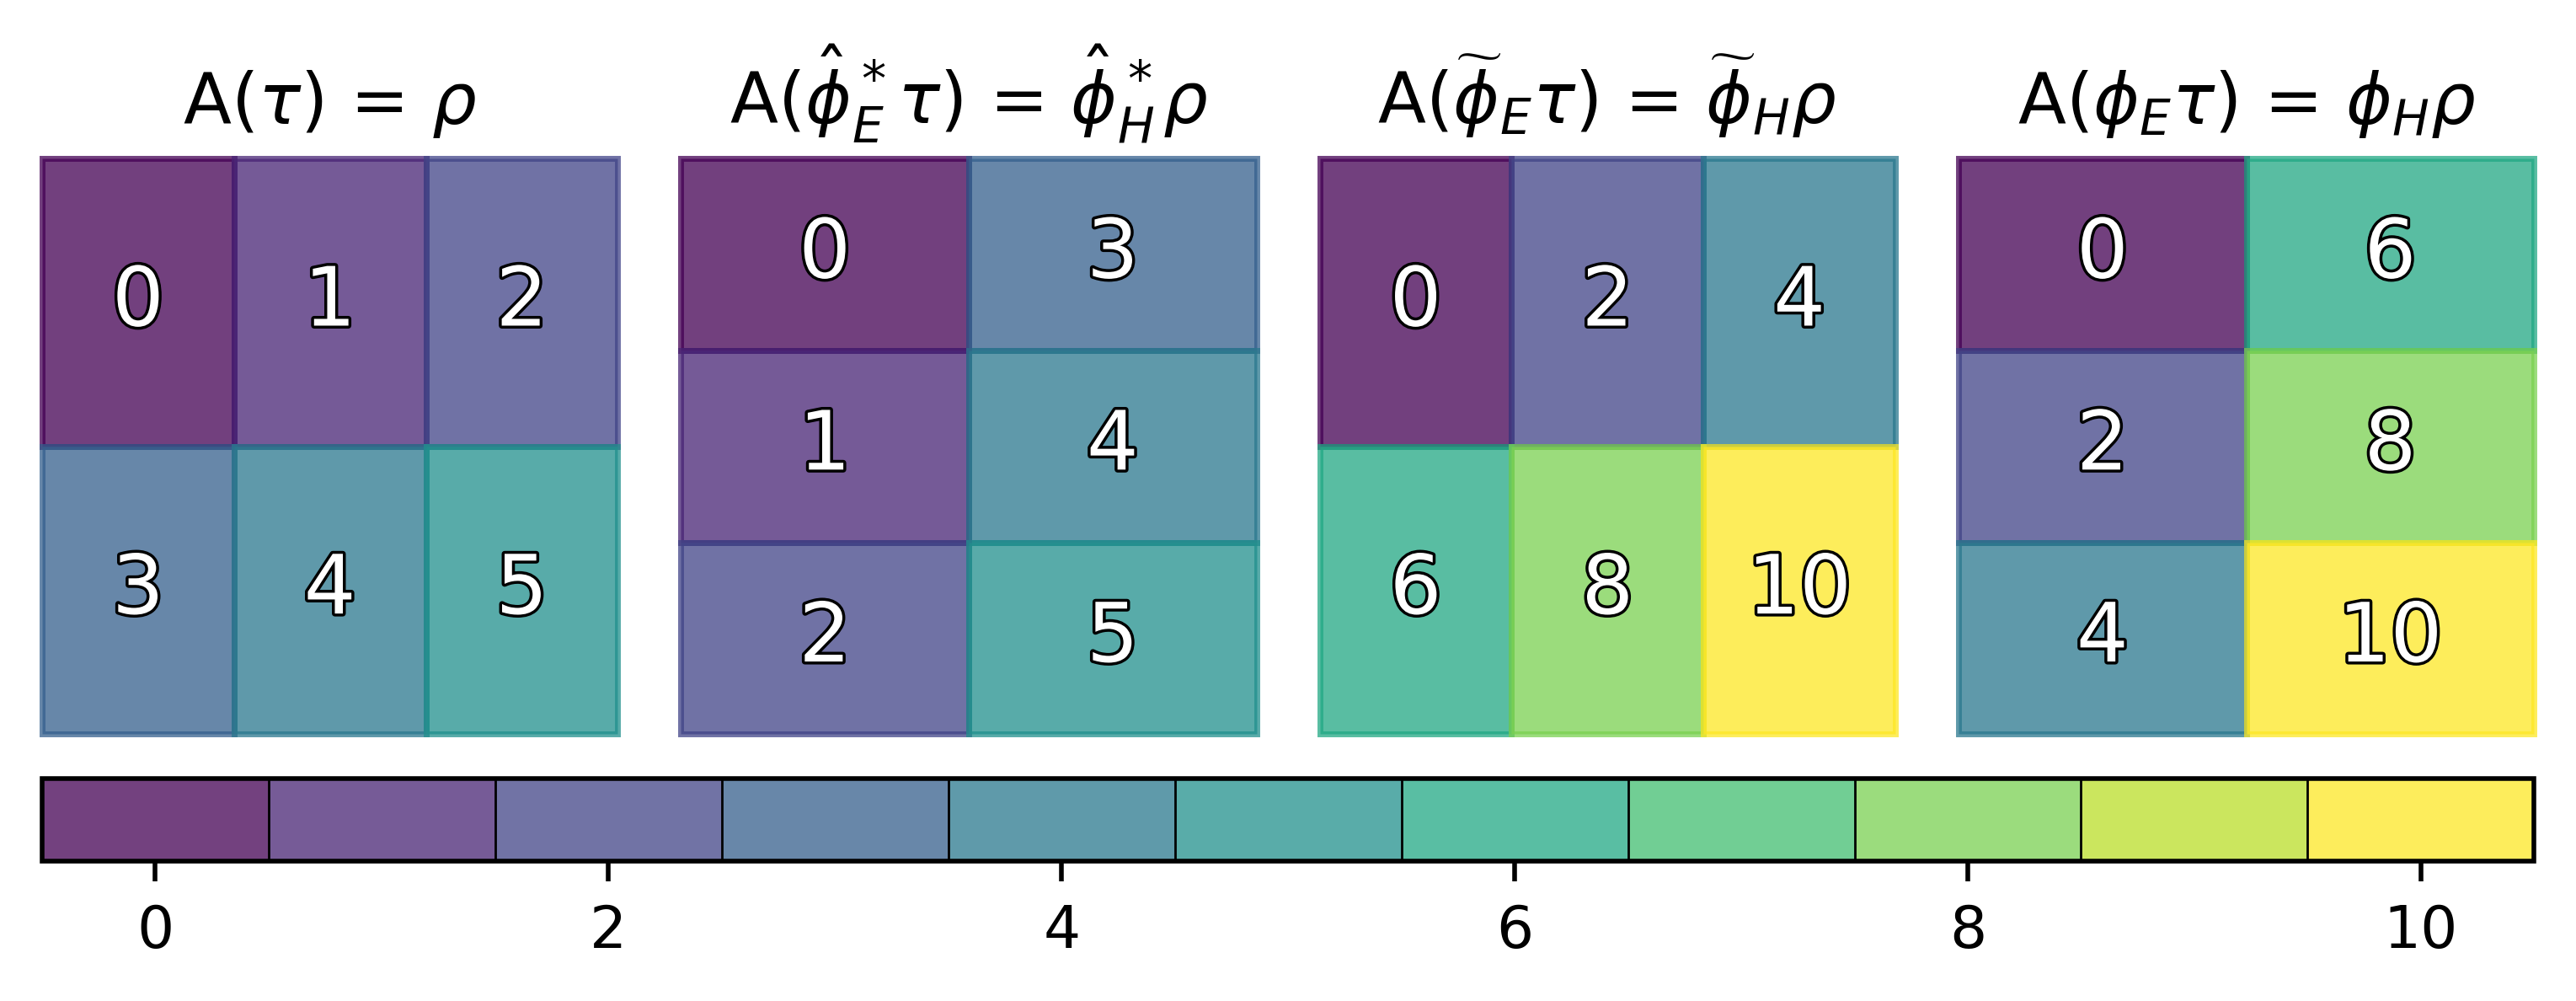
\includegraphics[width=1\columnwidth]{equivariance.png}
  \caption{}
\end{figure}
For example, in \autoref{fig:artist:equivarance}, the measurable variable is color. This is a visual representation of the data shown in \autoref{fig:atct:phi}, and as such the equivariant transformations are an equivalent transposition and scaling of the colors. This visualization is equivariant with respect to base space transformations, as defined in \autoref{eq:atct:equivarance:verify:base}, because the color values at the new position at the old position $measure_\dbasepoint^{\prime} = \measure_{\dbasepoint}$. This visualization is also equivariant with respect to fiber wise transformations, as defined in \autoref{eq:atct:equivarance:verify:fiber}, because the colors are consistently scaled in the same was the data. For example, the values that have become 2 and 4 in the $\dfunctc$ and $\dfunc$ panels are colored the same as the original 2 and 4 values in the first panel. The equivariance in this visualization is composable, as shown in the colors being both transposed and scaled correctly in the $\dfunc$ panel.

\subsection{Artist Operators}\label{sec:artist:operators}
A common use of category theory in software engineering is the specification of modular components \cite{wielsManagementEvolvingSpecifications1998} such that we can build systems where the structure preserved by components is preserved in the composition of the components. This allows us to express that an artist that works on a dataset can be composed of artists that work on sub parts of that dataset. 
\begin{equation}
  \label{eq:artist:operator}
  \begin{tikzcd}[column sep=small]
      & \dfiberc^{a} \times_{\dfiberc^{c}} \dfiberc^{b} 
    \arrow[ld, "{\pi_{a\times b, a}}"', color=fiber] 
    \arrow[rd, "{\pi_{a\times b, b}}", color=fiber] & & 
    \dtotalc^{a} \oplus_{\dfiberc^{c}} \dtotalc^{b} 
    \arrow[ddd, "\pi"', color=total] \\
    \dfiberc^{a} 
    %\arrow[d, "\pi"', color=fiber] 
    \arrow[r, "{\pi_{a,c}}", color=fiber] 
    & \dfiberc^{c} & \dfiberc^{b} 
    %\arrow[d, "\pi", color=fiber] 
    \arrow[l, "{\pi_{b,c}}"', color=fiber] & \\
    \dbasec^{a} 
    \arrow[rd, "{\iota_{a, a+b}}"', color=base] 
    & \dbasec^{c} 
    \arrow[r, "{\iota_{c,b}}", color=base] 
    \arrow[l, "{\iota_{c,a}}"', color=base] 
    & \dbasec^{b} 
    \arrow[ld, "{\iota_{b, a+b}}", color=base] 
    &  \\
    & \dbasec^{a}\sqcup_{\dbasec^c}\dbasec^{b} & & 
    \dbasec^{a}\sqcup_{\dbasec^c}\dbasec^{b} 
    \arrow[uuu, "{\dsectionc^{a,b}}"', dashed, bend right, color=section]
  \end{tikzcd}
\end{equation}

\subsubsection{Addition: +}
\label{sec:artist:addition}
As illustrated in \autoref{eq:artist:operator}, data bundles can be combined by taking the disjoint  union of base spaces $\dbase^{a} \sqcup_{\dbase^c} \dbase^b$, where $\dbase^c$ is an overlap. When the fibers of each bundle are isomorphic $\dfiber^{a} \simeq \dfiber^{b}$, which we denote as $\dtotal$, this is analogous to adding more observations to a dataset. We propose an addition operator that states that an artist that takes in a dataset can be constructed using artists that take as inputs subsets of the dataset

\begin{equation*}
  \label{eq:artist:addition}
  \vartistc_{a+b}(\cgamma{\dbasec^{a} \sqcup_{\dbase^c} \dbasec^b}{\dtotalc}) \coloneqq \vartistc_{a}(\cgamma{\dbasec^{a}}{\dtotalc}) + \vartistc_{b}(\cgamma{\dbasec^{b}}{\dtotalc}) 
\end{equation*}
As introduce in $\autoref{eq:artist:hom_transport}$, the artist returns a function $\gsection$. We assume that the output space is a trivial bundle, which means that $\gsectionc \in Hom(\gbase, \gfiber)$ because the output specification is the same at each point $\gbase$. This allows us to make use of the hom set adjoint property\note{find citation}\
\begin{equation*}
  Hom(\gbase^{a} + \gbasec^b, \gfiber) = Hom(\gbase^{a}, \gfiber) + Hom(\gbase^b, \gfiber)
\end{equation*} 
to define an artist constructed via addition as consisting of two distinct graphic sections
\begin{equation}
  \label{eq:artist:plus:output}
  \gsectionc(\gbasepointc) \coloneqq \begin{cases} \gsectionc^{a}(\gbasepointc) & \gbasepointc \in \vindexprec(\dbasec^{a}) \\
    \gsectionc^{b}(\gbasepointc) & \gbasepointc \in \vindexprec(\dbasec^{b})
  \end{cases}
\end{equation}
that are evaluated only if the input graphic point is an the graphic area that graphic section acts on. 

One way to verify that these artists are composable is to check that the return the same graphic on points in the intersection $\dbase^{c}$.  Given $\dbasepointc_{a} \in \dbasec_{c} \subset \dbasec_{a}$ and $\dbasepointc_{b} \in \dbasec_{c} \subset \dbasec_{b}$, if $\dbasepointc_{a} = \dbasepointc_{b}$ then

\begin{equation}
  \label{eq:artist:plus:verify}
  \begin{split}
  \vartistc_{a+b}(\dsectionc^{a+b}(\dbasepointc_{a})) \\ 
  = \vartistc_{a}(\dsectionc^{a}(\dbasepointc_{a})) = \vartistc_{b}(\dsectionc^{b}(\dbasepointc_{b}))
  \end{split}
\end{equation}
 for all $\dbasepointc_{a}, \dbasepointc_{b} \in \dbasec_{a}\bigsqcup\limits_{\dbasec_{c}} \dbasec_{b}$  
 
 One example of an artist that is a sum of artists is a sphere drawer that draws different quadrants of a sphere $\vartist(\dsection) = \vartist_{1}(\dsection_{1}) + \vartist_{2}(\dsection_{2}) + \vartist_{3}(\dsection_{3}) \vartist_{4}(\dsection_{4})$. Given an input $\dbasepoint \in \dbase_4$ in the 4th quadrant, then the graphic section that would be executed is $\gsection_{4}$. If that point is also in the 3rd quadrant  $\dbasepoint \in \dbase_3$, then both artist outputs must return the same values $\gsection_{4}(\vindexprec(\dbasepoint)) = \gsection_{3}(\vindexprec(\dbasepoint))$. 


\subsubsection{Multiplication: $\times$}
As illustrated in \autoref{eq:artist:operator},  fibers that are a cartesian product of fiberspaces $\dfiber^{a} \times_{\dfiber^c} \dfiber^{b}$, where $\dfiber^c$ is any fiber that is present in both fibers, can be projected down into component fibers. In the trivial case where the base spaces are the same $\dbase^{a} = \dbase^{b} = \dbase$, this is equivalent to adding more fields to a dataset. 

\begin{equation*}
  \label{eq:artist:multiplication}
  \vartistc_{a \times b}(\cgamma{\dbase}{\dtotalc^{a\times b}}) \coloneqq \vartistc_{a}(\cgamma{\dbasec}{\dtotalc^{a}}) \times \vartistc_{b}(\cgamma{\dbasec}{\dtotalc^{b}}) 
\end{equation*}
which following from an adjoint property of homsets \note{find citation}
\begin{equation*}
  Hom(\gbase, \gfiber) \times Hom(\gbase, \gfiber) = Hom(\gbase, \gfiber\times \gfiber)
\end{equation*}
which means that the artists on the subsets of fibers can be defined 
\begin{equation}
  \gsectionc^{a \times b} = \{\gsectionc^{a}(\gbasepointc), \gsectionc^{b}(\gbasepointc)\}, \gbasepointc \in \vindexprec(\dbasec)
\end{equation} 
but that the signature of $\gsectionc^{a \times b}$ would be $\gbase \rightarrow \gfiber \times \gfiber$. Instead of having to special case the return type of artists that are compositions of multiple case, the hom adjoint \note{find cite} property
\begin{equation*}
  Hom(\gbase, \gfiber \times \gfiber) = Hom(\gbase+\gbase, \gfiber)
\end{equation*}
 means that multiplication can be considered as a special case of addition where $\dbase^{a} = \dbase^{b}$. While we discussed the trivial case in \autoref{sec:artist:addition}, there is no strict  requirement that $\dfiber^{a} = \dfiber^{b}$. 

One way to verify that these artists are composable is to check that they encode any shared fiber $\dfiber^{c}$ in the same way.

\begin{equation}
  \begin{split}
    \extractmc(\vartistc_{a\times b}(\dsectionc^{a\times b}(\dbasepointc)))\restriction_{dfiberc^{c}}\\ = 
    \extractmc(\vartistc_{a}(\dsectionc^{a}(\dbasepointc_{a})))\restriction_{\dfiber^{c}} = \extractmc(\vartistc_{b}(\dsectionc^{b}(\dbasepointc_{b})))\restriction_{\dfiber^{c}}
  \end{split}
\end{equation}

This expectation of using the same encoding for the same variable is a generalization of the concept of consistency checking of multiple view encodings discussed by Zening and Hullman \cite{hullmanKeeping2018}. This expectation can also be used to check that a multipart glyph is assembled correctly. For example, a box plot \cite{wickham40YearsBoxplots2011} typically consists of a rectangle, multiple lines, and scatter points; therefore a boxplot artist $\vartist_{boxplot} = \vartist_{rect} \times \vartist_{errors} \times \vartist_{line} \times \vartist_{points}$ must be constructed such that all the sub artists draw a graphic at or around the same x value. 
\note{maybe stripped down box figure}


\section{Construction}
\label{sec:construction}
\subsection{Measurable Visual Components}

\begin{equation}
  \vfiberc \hookrightarrow \vtotalc \xrightarrow{\pi} \dbasec
\end{equation}
where
\begin{equation}
\cgamma{\opensetc}{\vtotalc\restriction_{\opensetc}} \coloneqq \big\{\vsectionc: \opensetc\rightarrow \vtotalc\restriction_{\opensetc} \; \bigm{\vert} \pi(\vsectionc(\dbasepointc)) = \dbasepointc\;for\, all\; \dbasepointc \in \opensetc \big\} 
\end{equation}

The bundle $\vtotal$ is structurally equivalent to the bundle $\dtotal$, but allows for separating the data that is input into the artist $\dsection$ from the data internal to the artist $\vsection$. This separation also allows for defining many of the target measurements \measure\ and the equivariant transformations to the measurements as internal components of the artists. 

\subsection{$\vindexc: \gbasec \rightarrow \dbasec$}
We define the functor $\vindex$ such that the data base space \dbase\ is a deformation retraction\cite{nlab:deformation_retract} of the graphic space $\gbase$, meaning that there is a continuous surjective mapping from every point $\dbasepoint\in\dbase$ to a point $\dbasepoint \in dbase$ . To simplify matters, in this paper, we construct the graphic space as a constant multiple of the base space such that 
\begin{equation}
  \underbrace{\opensetc\times[0,1]^{n}}_{\opensetgc} \textcolor{functor}{\xmapsto{\hspace{1em}\vindexc\hspace{1em}}} \opensetc 
\end{equation}
\begin{equation*}
  n = \begin{cases}
    dim(\gbase) - dim(\dbase) & dim(\dbase)<dim(\gbase)\\
  0 & otherwise
  \end{cases}
\end{equation*}

\subsection{Transforming Data into Measurable Components}
The transformation $\vchannel$ is a map from data sections to graphic sections
\begin{equation}
\nu: \cgamma{\opensetc}{\dtotalc\restriction_{\opensetc}} \rightarrow \cgamma{\opensetc}{\vtotalc\restriction_{\opensetc}}
\end{equation}
such that the sections project to the same point on the base space $\pi(\dtotal) = \pi(\vchannel(\dtotal))$. As with artists, $\vchannel$ are maps of sections such that the composition operators defined in \autoref{sec:artist:composition} can also act on transformers $\vchannel$. 

A consequence of $\pi(\dtotal) = \pi(\vchannel(\dtotal))$ is that $\vchannelc$ can be constructed as a pointwise transformation such that  
\begin{equation}
  \label{eq:constrution:nu}
  \vchannelc: \dfiberc_{\dbasepointc} \rightarrow \vfiberc_{\dbasepoint}
\end{equation}
which means that means that a point in a single data fiber $\delement \in \dfiber_{\dbasepointc}$ can be mapped into a corresponding point in a visual fiber $\velement \in \vfiber_{\dbasepointc}$. Since $\vchannel$ can be constructed as a pointwise function property, we can construct $\vchannelc$ functions 
\begin{equation}
  \label{eq:construction:nu:fabrication}
  \begin{tikzcd}[col sep=Huge]
    \dfiberc_{\dbasepointc} 
    \arrow[rr, "\vchannelc", color=artist] 
    \arrow[rrrr, "\vchannelc^{\prime\prime}", dashed, bend right, color=artist] &  & 
    \vfiberc_{\dbasepointc}\coloneqq{\dfiberc_{\dbasepointc}^{\prime}} 
    \arrow[rr, "\vchannelc^{\prime}", color=artist] &  & 
    \vfiberc^{\prime}_{\dbasepointc}
  \end{tikzcd}
\end{equation}
such that any new $\vchannel$ can be constructed as a composition of two or more $\vchannel$s. 

\subsubsection{Transformer Equivariance}

A pair of transformations $(\vchannel, \vchannel^{\prime})$ are equivariant if 
\begin{equation}
  \dfunct_{\vtotal} \vchannel(\dsection(\dbasepoint)) = \vchannel(\dfunct_{\dtotal}(\dsection(\dbasepoint)))
\end{equation}
for all $\dbasepoint \in \dbase$.  Since the visual sections and data sections are over the same space $\dfunc$

\begin{equation}
  \label{def:construction:nu:validate}
  \begin{tikzcd}[column sep=4em]
    {\dfiberc_{\dbasepointc}^{a}} \times {\dfiberc_{\dbasepointc}^{b}} 
    \arrow[d, "\pi_a"', color=fiber] 
    \arrow[r, "\vchannelc_{ab}", color=artist] 
    \arrow[rr, "\equivc_{ab}", bend left, color=monoid]  & 
    {\vfiberc_{\dbasepointc}^{a}} \times {\vfiberc_{\dbasepointc}^{b}} 
    \arrow[d, "\pi_a", color=fiber] & 
    \measurec_{\dbasepointc}^{ab} 
    \arrow[d, "\measurec\restriction_a", color=set] \\
    \dfiberc_{\dbasepointc}^a 
    \arrow[r, "\vchannelc_{a}", dashed, color=artist] & 
    \vfiberc_{\dbasepointc}^a 
    \arrow[r, "\simeq", dotted]  & 
    \measurec_{\dbasepointc}^a   \\
    {\dfiberc_{\dbasepointc}^{a}} \times {\dfiberc_{\dbasepointc}^{c}} 
    \arrow[u, "\pi_a", color=fiber] 
    \arrow[r, "\vchannelc_{ac}", color=artist] 
    \arrow[rr, "\equivc_{ac}", bend right, color=monoid] & 
    {\vfiberc_{\dbasepointc}^{a}} \times {\vfiberc_{\dbasepointc}^{c}} 
    \arrow[u, "\pi_a"', color=fiber] & 
    \measurec_{\dbasepointc}^{ac} 
    \arrow[u, "\measurec\restriction_a"', color=set]            
    \end{tikzcd}
\end{equation}

\subsection{Compositing Measurable Components into Output}
The compositing function $\vmarkc$ transforms the sections of visual elements $\vsectionc$ into sections of graphics $\gsectionc$.
\begin{equation}
  \vmarkc: \cgamma{\opensetc}{\vtotalc\restriction_{\opensetc}} \rightarrow \cgamma{\opensetgc}{\gtotalc\restriction_{\opensetgc}}
\end{equation}

\begin{equation}
  \label{eq:construction:q:fabrication}
  \begin{tikzcd}
      \cgamma{\opensetc}{\vtotalc\restriction_{\opensetc}} 
      \arrow[rr, "\vchannel", color=artist] 
      \arrow[rrrr, "\vmarkc^{\prime}"', bend right, color=artist, dashed] &  & \cgamma{\opensetc}{\vtotalc^{\prime}\restriction_{\opensetc}} 
      \arrow[rr, "\vmarkc", color=artist] &  & \cgamma{\opensetgc}{\gtotalc\restriction_{\opensetgc}}
      \end{tikzcd} 
\end{equation}

\subsubsection{Compositor Equivariance}

As mentioned in \autoref{sec:construction:nu}, the distinction between data sections $\dsection$ and visual sections $\vsection$ is semantic rather than structural. Therefore, the equivariance condition on the sheaf map with a change of base space $\vmarkc$ is identical to the one for artists shown in \autoref{eq:artist:equivariance} such that an equivariant \vmark\ must satisify the condition 
\begin{equation}
  \vmarkc(\dfunctc_{\vtotalc}(\vsectionc(\dfunchc_{\vtotalc}(\vindexc(\gbasepointc^{\prime}))))) = \dfunctc_{\gtotalc}(\vmarkc(\vsectionc(\vindexc(\dfunchc_{\gtotalc}(\gbasepointc^{\prime})))))  
\end{equation}
which means that any change to a measurable component input must have a measurably equivalent change in the output. 

As with the artist, it is difficult to work with the output section \gsection\ directly and instead we test the compositer \vmark\ using measurements derived from the output. A compositer is expected to pass visual transformers \vsection\ through to their expected visual measurements, as described in \autoref{def:construction:nu:validate}, such that any shared visual components at a point $\vsection^{a}(\dbasepoint)$ must render to the same measurement $\measure^{a}_{\dbasepoint}$
\begin{equation}
  \label{eq:construction:q:validate}
  \begin{tikzcd}[row sep=huge]
    \cgamma{\opensetc}{(\vtotalc^{a}\times \vtotalc^{b})\restriction_{\opensetc}}  
    \arrow[rr, "\vmarkc_{ab}", color=artist] \arrow[d, "\pi_a"', color=total] &  &  \imartistsub{ab}{\opensetgc}{\gtotalc\restriction_{\opensetgc}} 
    \arrow[d, "\measurec\restriction_a \circ \extractmc_{ab}", color=monoid]  \\
   \cgamma{\opensetc}{\vtotalc^{a}\restriction_{\opensetc}} 
   \arrow[rr, "\simeq", dotted] &  & {\textcolor{set}{Hom}(\opensetc, \measurec^{a})}                                                                             \\
    \cgamma{\opensetc}{(\vtotalc^{a}\times \vtotalc^{c})\restriction_{\opensetc}}  \arrow[rr, "\vmarkc_{ab}", color=artist] \arrow[u, "\pi_a", color=total]  &  &  \imartistsub{ac}{\opensetgc}{\gtotalc\restriction_{\opensetgc}} \arrow[u, "\measurec\restriction_a \circ \extractmc_{ac}"', color=monoid]
   \end{tikzcd}
\end{equation}


\note{when $Q_{ab} = Q_{bc}$, this says only things that change are the parameter controlled pieces}

\subsection{Constructing the Artist: $\vartistc=\vmarkc\circ\vchannelc$}

As shown in \autoref{eq:atct:sheaves:homset}, sheaves equipped with transport functors have isomorphic maps between the sheaves. This property, allows us to specify the transformation from data to graphic space in data or graphic space or a combination, as listed in \autoref{eq:artist:hom_transport}, such that the following diagram commutes:
\begin{equation}
  \label{eq:construction:artist:path}
\begin{tikzcd}[row sep=2.5em, column sep=1.5em]
  \cgamma{\opensetc}{\dtotalc\restriction_{\opensetc}} 
  \arrow[rr, "\vchannelc^{\dbasec}", color=artist] 
  \arrow[rrrr, "\vartistc^{\dbasec}", bend left, color=artist] 
  \arrow[dd, "\vindexpullc"', color=functor] 
  \arrow[rrrrdd, "\vartistc", color=artist, pos=.2] &  & 
  \cgamma{\opensetc}{\vtotalc\restriction_{\opensetc}} 
  \arrow[rrdd, "\vmarkc", color=artist] 
  \arrow[rr, "\vmarkc^{\dbasec}", color=artist] 
  \arrow[dd, "\vindexpullc", color=functor, pos=.2] &  & \imartist{\opensetc}{\vindexpushc\gtotalc\restriction_{\opensetc}}  \\
   & & & & \\
  \cgamma{\opensetgc}{\vindexpullc\dtotalc\restriction_{\opensetgc}} \arrow[rr, "\vchannelc^{\gbasec}", color=artist] 
  \arrow[rrrr, "\vartistc^{\gbasec}", bend right, color=artist] & & 
  \cgamma{\opensetgc}{\vindexpullc\vtotalc\restriction_{\opensetgc}} \arrow[rr, "\vmarkc^{\gbasec}", color=artist] &  & 
  \imartist{\opensetgc}{\gtotalc\restriction_{\opensetgc}} \arrow[uu, "\vindexpushc"', color=functor]
\end{tikzcd}  
\end{equation}
The diagram in \autoref{eq:construction:artist:path} illustrates how a developer can connect transformations over data space, denoted with a subset $\dbase$, with transformations over graphic space $\gbase$, using $\vindexpushc$ and $\vindexpullc$ adaptors. This allows developers to for example connect transformers that transform data on a line to a color in dataspace, but build a line compositing function that dynamically resamples what is on screen in graphic space. x

\section{Discussion}
\subsection{Limitations}
\subsection{future work}

\section{Conclusion}
The conclusion goes here.


\appendices



% use section* for acknowledgment
\ifCLASSOPTIONcompsoc
  % The Computer Society usually uses the plural form
  \section*{Acknowledgments}
\else
  % regular IEEE prefers the singular form
  \section*{Acknowledgment}
\fi


The authors would like to thank...


% Can use something like this to put references on a page
% by themselves when using endfloat and the captionsoff option.
\ifCLASSOPTIONcaptionsoff
  \newpage
\fi

% trigger a \newpage just before the given reference
% number - used to balance the columns on the last page
% adjust value as needed - may need to be readjusted if
% the document is modified later
%\IEEEtriggeratref{8}
% The "triggered" command can be changed if desired:
%\IEEEtriggercmd{\enlargethispage{-5in}}

% references section

% can use a bibliography generated by BibTeX as a .bbl file
% BibTeX documentation can be easily obtained at:
% http://mirror.ctan.org/biblio/bibtex/contrib/doc/
% The IEEEtran BibTeX style support page is at:
% http://www.michaelshell.org/tex/ieeetran/bibtex/
\bibliographystyle{IEEEtran}
% argument is your BibTeX string definitions and bibliography database(s)
\bibliography{bibliography}

% biography section 
% If you have an EPS/PDF photo (graphicx package needed) extra braces are
% needed around the contents of the optional argument to biography to prevent
% the LaTeX parser from getting confused when it sees the complicated
% \includegraphics command within an optional argument. (You could create
% your own custom macro containing the \includegraphics command to make things
% simpler here.)
%\begin{IEEEbiography}[{\includegraphics[width=1in,height=1.25in,clip,keepaspectratio]{mshell}}]{Michael Shell}
% or if you just want to reserve a space for a photo:

%\begin{IEEEbiography}{Michael Shell}
%\end{IEEEbiography}

% if you will not have a photo at all:
\begin{IEEEbiographynophoto}{Hannah Aizenman}
Biography text here.
\end{IEEEbiographynophoto}

\begin{IEEEbiographynophoto}{Thomas Caswell}
  Biography text here.
\end{IEEEbiographynophoto}
% insert where needed to balance the two columns on the last page with
% biographies
%\newpage

\begin{IEEEbiographynophoto}{Michael Grossberg}
Biography text here.
\end{IEEEbiographynophoto}

% You can push biographies down or up by placing
% a \vfill before or after them. The appropriate
% use of \vfill depends on what kind of text is
% on the last page and whether or not the columns
% are being equalized.

%\vfill

% Can be used to pull up biographies so that the bottom of the last one
% is flush with the other column.
%\enlargethispage{-5in}

% that's all folks
\end{document}


